\documentclass{article}

%%% Fill details here (in the second brackets)
\newcommand{\name}{Kaushik Dutta and Sung Min Ha}     % Your name (First Last)
\newcommand{\wustlkey}{CSE515T 2021 Final Project Report}             % Your WUSTL Key
%%%



%%%%%%%%%%%%%%%%%%%%%% Formatting Stuff %%%%%%%%%%%%%%%%%%%%%%%%%%%
\usepackage{times}
\usepackage[T1]{fontenc}


\setlength{\parskip}{1em}\setlength{\parindent}{0pt}
\linespread{1.25}
\usepackage[margin=0.7in,top=1in]{geometry}\usepackage{fancyhdr}
\pagestyle{fancy}\lhead{\bf \name}\rhead{\bf \wustlkey}\cfoot{\thepage}
\newcommand{\info}{\clearpage \subsection*{Information}}
\newcommand{\solution}[1]{\clearpage \subsection*{Solution #1}}
\newcommand{\spart}[1]{\paragraph{(#1)}}
%%%%%%%%%%%%%%%%%%%%%%%%%%%%%%%%%%%%%%%%%%%%%%%%%%%%%%%%%%%%%%%%%%%


%%% Add any more packages if you want to
\usepackage{amsmath,graphicx}

\title{Predicting English Premier League match results using Bayesian Hierarchical Model}

\begin{document}

\maketitle

\section{Introduction}
The statistical modelling of sports data has become increasingly popular in the last few years after the advent of machine learning which gives the ability to construct predictive models with unprecedented accuracy. For ages the betting companies have employed statistical intuition based on the team’s performance to calculate odds for predicting football results. But the biggest challenge in accurately predicting the results of a football match are the uncertainty pertaining to the results and thus it cannot be realized by a linear model. The football results prediction is based on complex non linear parameters encompassing a team’s performance over a varying timeframe and depending on a wide range of factors ranging from player performance statistics to home field advantage. To accommodate the non-linearity of the data, we propose a Bayesian Hierarchical Model that can be employed to predict the ranking of the English Premier League season alongwith a prediction of results and scores of a particular match in the season. A major reason behind choosing English Premier League is because it is highly competitive in nature and there is a high incidence of upsets (where weak teams outscore strong teams). The world was awed when the football club Leicester City won the championship in 2016, against all odds, but this demonstrates the highly unpredictable nature of the game, and therefore the difficulty of the problem we are trying to tackle.

\section{Method}

\subsection{Dataset and Preprocessing}
For this project we considered the English Premier League 2017-2018 season data. The English Premier League is the first division football league of the UK contested by 20 teams where each team plays against each other twice ( home and away ). A total of 380 matches are played in a season and the team with the highest point is declared winner. The top four teams of the league table goes on to play UEFA Champions League. The next three teams qualify for the Europa League and the bottom three teams are relegated to the Second Division league. We obtained our dataset from http://www.football-data.co.uk/data.php. The dataset has match statistics for all the matches in the season in terms of goals scored, corners, shots , fouls , red and yellow cards for both home and away teams. For preprocessing we trimmed the dataset to only include features which directly or indirectly affects the final match results and arranged the matches in a longitudinal fashion according to their dates.

\subsection{Feature Selection and Feature Engineering}
The quality of results in the prediction task is directly associated to the quality of the feature set used for modelling the system hence choosing the right features is of paramount importance. We divided the available features into two categories : 1) Attack and Defence Parameters consisting of the feature like goals scored and full/half time results which directly affect the match results and 2) Indirect Features consisting of the feature like corners, fouls, shots etc which provides us with mathematical insights regarding team performance and influence the match result in an indirect way. 
    When designing our model’s features for the prediction of football results, we wanted to introduce features that could provide us with useful quantifiable insights for judging the recent performance of a team. To this end we engineered two unique features called Form and Streak. These features enhance the predictive power of the model by incorporating the fact that recent performance of the team has the ability to influence the current game. The mathematical formulation for the engineered features are given as :

\subsubsection{Streak}
This feature encapsulates the recent improving/declining trend in the performance of a team. The Streak value for a team is computed by assigning a score to each match result and taking the mean of the previous k scores, where k is a hyper-parameter. We also included a temporal dimension to the Streak feature by placing time-dependent weights on the scores of the previous games of a team, obtaining a feature that we refer to as the Weighted Streak (greater weights for recent games, decreasing gradually for non-recent games).

\begin{equation}
\delta_j = \Sigma_{p=j-k}^{j-1} \frac{2(p-(j-k-1) res_{p}}{3k(k+1)}
\label{eq:streak}
\end{equation}

where, $\delta_j$ is the Weighted Streak of a team in the $j$-th match and the resp is point each team gets as per the result of the match (0-Loss, 1-Draw , 3-Win)

\subsubsection{Form}
This feature encapsulates the recent performance of the team relative to its opponents. The Form value of each team is initialized to one at the beginning of each season and then updated after each match according to the result of the match i.e. win,draw,loss. Our mathematical formulation of Form ensures that a greater coefficient update is provided if a weak team triumphs over a strong team, and vice-versa. In the case of a draw, the Form of a weak team increases while that of a strong team decreases. 
When a team $\alpha$ beats $\beta$ we can write the Form ($\xi$) equation for the teams as:
\begin{equation}
\xi_{j}^{\alpha}= \xi_{j-1}^{\alpha}  + \gamma\xi_{j-1}^{\beta}
\label{eq:form_1}
\end{equation}
\begin{equation}
\xi_{j}^{\beta}= \xi_{j-1}^{\beta}  - \gamma\xi_{j-1}^{\beta}
\label{eq:form_2}
\end{equation}
where $\gamma$ is the stealing fraction signifying the weight to be added/subtracted in case of win/loss

\begin{equation}
log \theta_{g1} = home + att_{h(g)} + def_{a(g)} + intercept
\label{eq:log_g1}
\end{equation}

\begin{equation}
log \theta_{g2} = att_{a(g)} + def_{h(g)} + intercept
\label{eq:log_g2}
\end{equation}

\subsubsection{Model Description}



\section{Results}

%\begin{figure*}[!htb]
 % \centering
%  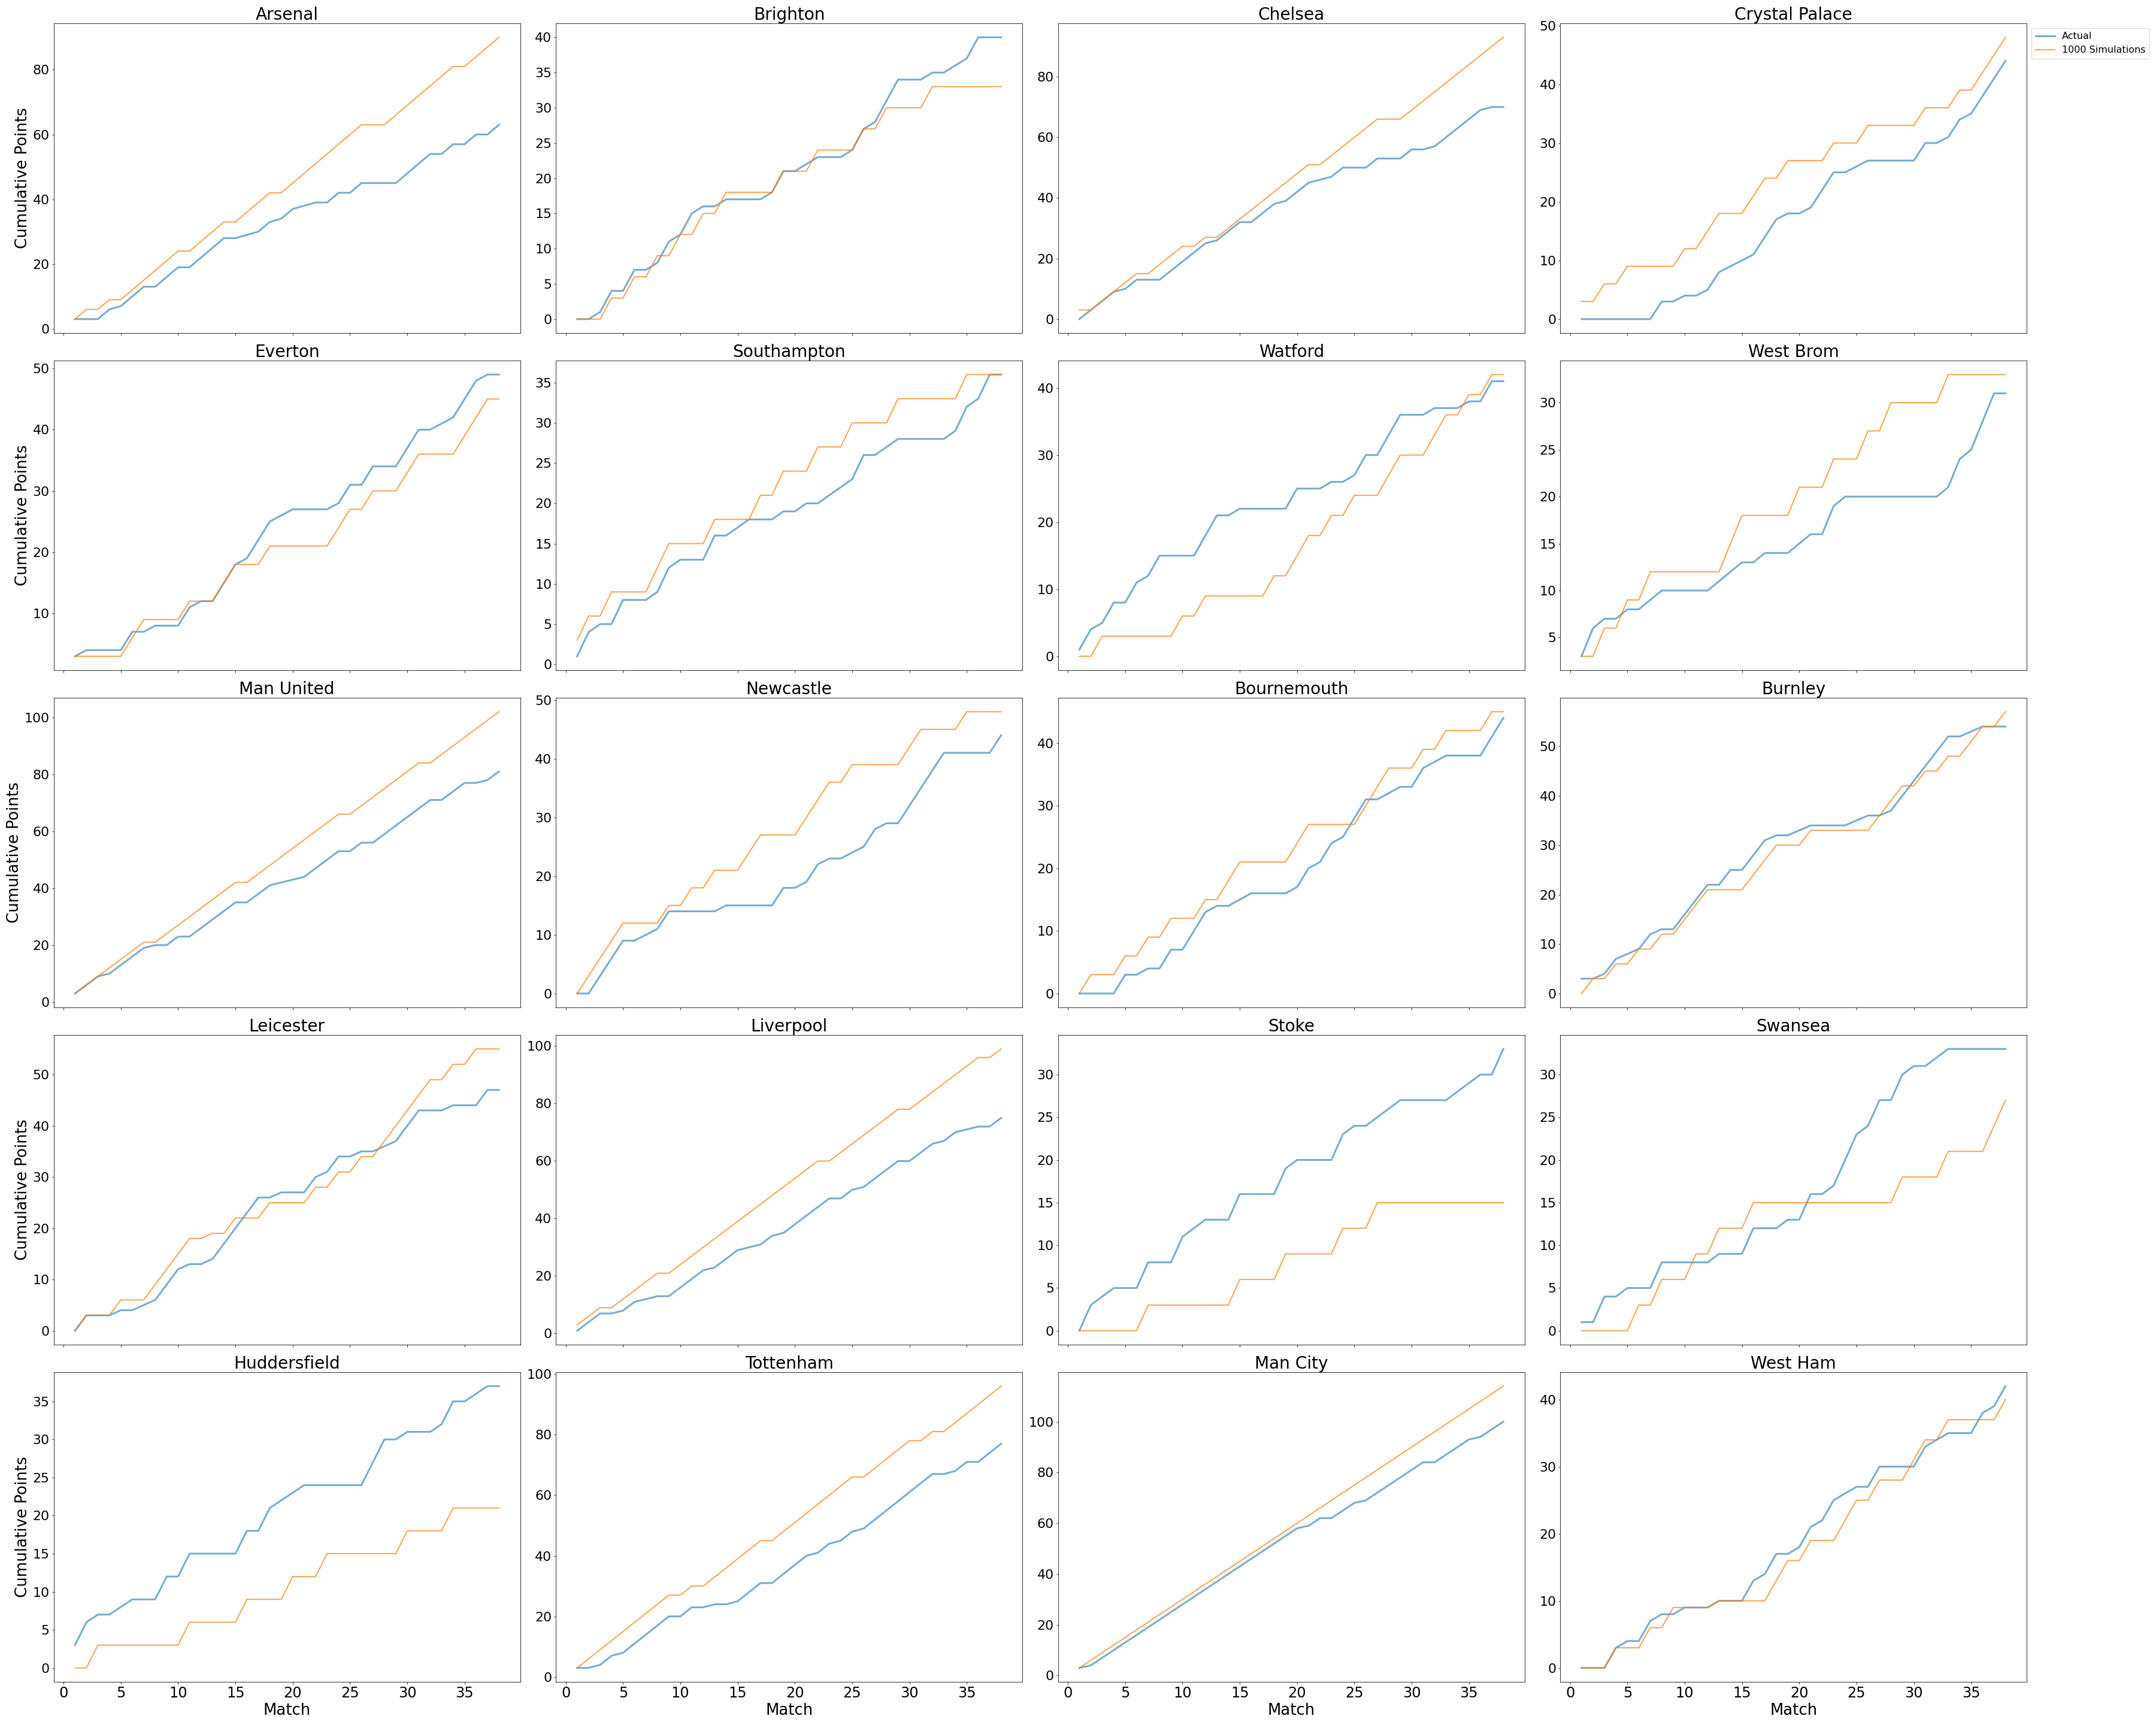
\includegraphics[width=40em]{charts_20210505_005741/Actual_vs_Prediction_Per_Match_Points_Team_4000_20.png}
%  \caption{Problem 1d. K3}
%  \label{fig:1d_3}
%\end{figure*}



\section{Conclusion}



\end{document}
